\section{Database Approach - Examples}

    This section is meant to explain how to model a tree after ones liking,
    using the database-approach. As stated priviously, the seed is determined by
    a stream of (interface, node) tuples which define the branching/leaf-levels
    of the tree.

\subsection{Basemodel}

    To start off, a base-tree is considered from which specialized instances
    will be derived. \\
                                             
\begin{tabular}{ll}
  &StdEarth\\
  <<.&(strif, strbranch)\\
  .<<&(leafif 0.1, stdleaf 1.0 1.1)\\
\end{tabular}
 
\begin{figure}[htb]
        \centering
        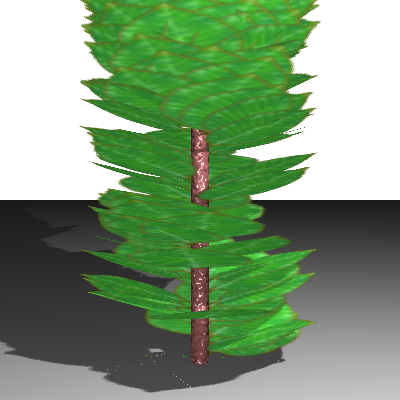
\includegraphics[height=4cm,width=4cm, angle=0]{images/dbex0}
        \caption{The basic building-blocks}
        \label{fig:graph2}
\end{figure}

    Only two levels, one trunk and one leafnode results in the above image,
    using simple standard components, \emph{strif, strbranch} and the
    leaf-components \emph{leafif} (leaf interface) and \emph{stdleaf} which
    simply takes the size and a development parameter.

\subsubsection{Adding branches}

    Adding branches by placing a branch-level between the existing ones.

\begin{tabular}{ll}
  &StdEarth\\
  .<<&(if\_setdist (dist\_root 10.0 29.1) \$ strif,\\
  &br\_setthick 0.2 \$ strbranch)\\
  <<&(angif 90 0,\\
  &br\_setthick 0.2 \$ strbranch)\\
  <<.&(if\_setevol (efnc\_param 0.05 0.0) \$ leafif 0.5,\\
  &stdleaf 4.0 0.10)\\
\end{tabular}

\begin{figure}[htb]
        \centering
        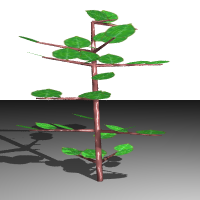
\includegraphics[height=4cm,width=4cm, angle=0]{images/dbex1}
        \caption{Another branch-level added}
        \label{fig:graph3}
\end{figure}

    Branches appear from the trunk and carries the leaf into the surrounding.
    Also note that the \emph{if\_setdist} sets the distribution function, that
    is the function that says how power will be distributed on a certain level.
    the \emph{br\_setthick} sets the thickness of certain branch-level.

\subsubsection{Randomize}

    The branch interfaces have this far been static and will now be randomized.
    More branch-levels are added.

\begin{tabular}{ll}
    &StdEarth\\
    .<<&(if\_setdist (dist\_root 10.0 29.1) \$ strif,\\ 
    &br\_setthick 0.2 \$ ranagebranch 0.3 0.0)\\
    <<&(if\_setmod (mdfnc\_rlen 0.7)  \$ \\
    &if\_setevol (efnc\_param 0.5 0.2) \$ \\
    &if\_setdist (dist\_shaped 1.4 (\_->1.0) (16.0, 0.1) ) \$ \\
    &angifi 20 45 , \\
    &br\_setthick 0.1 \$ ranwigbranch 0.5 0.2)\\
    <<&(if\_setmod (mdfnc\_mplen 0.7)  \$ \\
    &if\_setevol (efnc\_param 0.14 0.01) \$ \\
    &if\_setdist (dist\_shaped 0.3 (\_->1.0) (7.0,1.0)) \$ \\
    &angifi 35 55 , \\
    &br\_setthick 0.1 \$ ranwigbranch 0.5 0.4) \\
    <<.&(if\_setevol (efnc\_param 0.05 0.0) \$ leafif 0.5, \\
    &stdleaf 4.0 0.10) \\
 
\end{tabular}

\begin{figure}[htb]
        \centering
        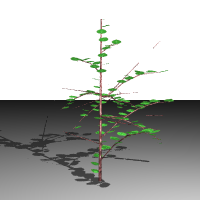
\includegraphics[height=4cm,width=4cm, angle=0]{images/dbex2}
        \caption{Randomization and some modifications added}
        \label{fig:graph4}
\end{figure}

    The \emph{if\_setmod} sets a restriction on the power distributed from a
    certain level. \emph{mdfnc\_rlen 0.7} says that a child cannot grow beyond
    0.7 times the relative growth of its mother. The \emph{if\_setevol} sets the
    evolution paramaters for a level, that is when it is going to spawn. Using
    ranwigbranch a complex multi-period sine-shape is applied to the branches.
    The \emph{if\_setshaped} is used to set the shape of a level. Typically on
    the trunk-level a certain shape is defined. For columnar trees such as this
    example, it may simply by a \emph{lambda}->1.0 to say that it branches should be
    equally intensified over the trunk, while some trees might have more of a
    pyramid or even wavy shape. The \emph{angifi x y} says that a branch will
    spawn with an angle of x +/- y in relation to its mother. 

\subsubsection{Further improvements}

    Adding more levels and fine-tuning the parameters gives further improvements
    to the scene.\\

\begin{tabular}{ll}
  &StdEarth\\
  .<<&(if\_setdist (dist\_root 10.0 29.1) \$ strif,\\
  &br\_setthick 0.1 \$ ranagebranch 0.3 0.0)\\
             
         <<&(if\_setmod (mdfnc\_rlen 0.7)  \$\\ 
           &if\_setevol (efnc\_param 0.5 0.2) \$\\ 
           &if\_setdist (dist\_shaped 1.4 f0 (16.0, 0.1) ) \$\\ 
           &angifi 20 45 ,\\ 
           &br\_setthick 0.1 \$ ranwigbranch 0.5 0.2)\\

         <<&(if\_setmod (mdfnc\_mplen 0.7)  \$ \\
           &if\_setevol (efnc\_param 0.14 0.01) \$ \\
           &if\_setdist (dist\_shaped 0.3 f0 (7.0,1.0)) \$ \\
           &angifi 35 55 , \\
           &br\_setthick 0.1 \$ ranwigbranch 0.5 0.4) \\
             
         <<&(if\_setmod (mdfnc\_mplen 0.1 ) \$ \\
           &if\_setevol (efnc\_param 0.05 0.005) \$ \\
           &if\_setdist (dist\_shaped 0.3 f0 (3.0,1.0)) \$ \\
           &angifi 45 65, \\
           &br\_setthick 0.1 \$ ranwigbranch 0.5 0.9) \\
         <<.&(if\_setevol (efnc\_param 0.05 0.0) \$ leafif 0.05, \\
            &stdleaf 4.0 0.10) \\
	
\end{tabular}


\begin{figure}[htb]
        \centering
        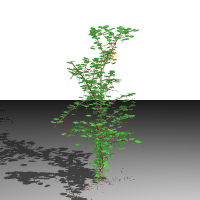
\includegraphics[height=4cm,width=4cm, angle=0]{images/dbex3}
        \caption{Randomization and some modifications added}
        \label{fig:graph5}
\end{figure}



      
